\documentclass[11pt]{article}
\usepackage[a4paper,margin=25mm]{geometry}
\usepackage{amsmath,amssymb,amsthm,mathrsfs,booktabs,graphicx,url}

% Rectangular highlights for the update rules used in the simulations.
\usepackage{xcolor,tcolorbox}
\definecolor{RuleGradient}{RGB}{27,96,143}
\definecolor{RuleNewton}{RGB}{157,77,37}
\definecolor{RuleDiagonal}{RGB}{17,120,99}
\definecolor{RuleIdentity}{RGB}{112,75,155}
\definecolor{RuleLoss}{RGB}{164,117,18}
\definecolor{RuleLeastSquares}{RGB}{81,96,113}
\newenvironment{updaterule}[2]{%
  \begin{tcolorbox}[
    colback=#1!6!white, colframe=#1!65!black,
    colbacktitle=#1!12!white, coltitle=#1!45!black,
    title={#2}, halign title=right,
    fonttitle=\normalfont\sffamily\bfseries\small,
    boxrule=.5pt, arc=0pt, outer arc=0pt,
    left=2mm, right=2mm, top=0mm, bottom=0mm,
    toptitle=1mm, bottomtitle=1mm,
    before skip=8pt, after skip=8pt]
}{\end{tcolorbox}}
\newtheorem{proposition}{Proposition}[section]
\newtheorem{corollary}[proposition]{Corollary}
\theoremstyle{remark}
\newtheorem{remark}{Remark}[section]
\setlength{\parindent}{1.2em}
\setlength{\parskip}{2pt}
\setlength{\emergencystretch}{1em}
\makeatletter
% Verified external numbers from the supplied revised manuscript.
% These definitions are for this standalone preview only.
\@namedef{r@subsec:OHAM_reformulation}{{3}{--}}
\@namedef{r@sec:problem_formulation}{{2}{--}}
\@namedef{r@eq:NOHAM_iterative_update}{{38}{--}}
\@namedef{r@eq:fsm_impulse_coefficients}{{C.5}{--}}
\@namedef{r@rem:fsm_innovation_energy}{{Appendix C.2}{--}}
\@namedef{r@app:fsm_innovation_energy}{{D}{--}}
\@namedef{r@sec:results}{{5}{--}}
\@namedef{r@eq:faa_di_bruno_particularized}{{E.7}{--}}
\@namedef{r@eq:next_inter_init_guess}{{37}{--}}
\@namedef{r@eq:NOHAM_HODE}{{33}{--}}
\@namedef{r@eq:NOHAM_residual}{{34}{--}}
\@namedef{r@eq:w_wiener_uv_theta_c}{{7}{--}}
\makeatother
\begin{document}
\begin{center}
{\large\bfseries Proposed replacement for Section 4 and associated appendices}
\end{center}
\noindent The main section and the additional appendices below are intended
for separate insertion into the revised manuscript. External references
retain the numbering in the supplied PDF; pagination here uses a standalone
article layout. Existing Appendices A--G are not reproduced.
\medskip
\setcounter{section}{3}
\setcounter{equation}{38}
\setcounter{table}{1}
\section{GOTHAM for Wiener systems with AR output noise}
\label{sec:GOTHAM_for_WS_AR_noise}

Now the operator-theoretic HAM formulation in Section~\ref{subsec:OHAM_reformulation} is particularized to the Wiener system with AR output noise formulated in Section~\ref{sec:problem_formulation}. The underlying Wiener operator in \eqref{eq:w_wiener_uv_theta_c} may be written formally as
\begin{equation}
    \mathcal{W}^{(u,\nu)}:\Theta\to Y,
\end{equation}
where the measured input realization $u$ and the innovation realization $\nu$ are fixed by the problem at hand. The innovation sequence is not available to the estimator. Therefore, the implementable identification problem must be formulated using the measured input $u$, the measured output samples $C$, and quantities reconstructed from the successive parameter estimates.

At iteration $k$, the current estimate $\hat{\theta}^{(k)}$ is used as the initial point of the local homotopy construction \eqref{eq:next_inter_init_guess}. Then, solving the HODE recursion~\eqref{eq:NOHAM_HODE} up to order $M$ gives the deformation terms $\{\theta_m^{(k)}\}_{m=1}^{M}$, and the parameter estimate is updated according to \eqref{eq:NOHAM_iterative_update}.

Colored boxes identify the implemented update configurations using the
acronyms in Section~\ref{sec:results}. The PL and FSM qualifiers distinguish
the parametrizations; a shared box lists the variants using the same
update form with different auxiliary operators.

Two implementable parametrizations are considered in this contribution. In the pseudo-linearized parametrization, the regressor matrix $\hat{\Phi}^{(k)}$ defined in Section~\ref{sec:problem_formulation} is kept fixed during the current parameter update. In the FSM parametrization, the identification criterion is defined through the energy of the candidate innovation residual, in agreement with the innovation-energy criterion stated in Remark \ref{rem:fsm_innovation_energy} and justified in Appendix~\ref{app:fsm_innovation_energy}.

\subsection{Pseudo-linearized parametrization}

\label{subsec:GOTHAM_PL_parametrization}

At iteration $k$, latent signals $\hat{\alpha}^{(k)}(t)$ and $\hat e^{(k)}(t)$ are reconstructed from the current estimate $\hat{\theta}^{(k)}$, yielding the estimated state matrix $\hat{\Phi}^{(k)}$. During the computation of the GOTHAM correction terms at iteration $k$, this matrix is frozen. Thus, the pseudo-linearized parameter-to-output map is
\begin{equation}
\label{eq:WS_pseudolinear_operator_k}
    \mathcal{W}_{\mathrm{PL}}^{(k)}(\theta)
    =
    \hat{\Phi}^{(k)}\theta.
\end{equation}

The least-squares loss is
\begin{equation}
\label{eq:WS_loss_k}
    J_{\mathrm{PL}}^{(k)}(\theta)
    =
    \frac{1}{2}
    \left\|
    C-\hat{\Phi}^{(k)}\theta
    \right\|_2^2.
\end{equation}
From those, define
\begin{equation}
\label{eq:WS_gradient_hessian_definitions}
    G^{(k)}
    :=
    \hat{\Phi}^{(k)\top}\hat{\Phi}^{(k)},
    \qquad
    b^{(k)}
    :=
    \hat{\Phi}^{(k)\top}C,
    \qquad
    g^{(k)}
    :=
    \nabla_{\theta}J_{\mathrm{PL}}^{(k)}(\hat{\theta}^{(k)})
    =
    G^{(k)}\hat{\theta}^{(k)}-b^{(k)}.
\end{equation}
Since $\hat{\Phi}^{(k)}$ is frozen during the current update, $J_{\mathrm{PL}}^{(k)}$ is quadratic in $\theta$. This permits explicit update formulas for the gradient-root and loss-root formulations.

\subsection{Gradient-root formulation for the pseudo-linearized parametrization}
\label{subsec:GOTHAM_PL_gradient_root}

In the gradient-root formulation, the residual operator is
\begin{equation}
\label{eq:gradient_root_operator}
    \mathcal{N}_{G,\mathrm{PL}}^{(k)}(\theta)
    =
    \nabla_{\theta}J_{\mathrm{PL}}^{(k)}(\theta)
    =
    G^{(k)}\theta-b^{(k)}.
\end{equation}

Thus, $\mathcal N_{G,\mathrm{PL}}^{(k)}:\mathbb R^n\to\mathbb R^n$.
Since this operator is affine, its residual coefficients and deformation
terms have simple expressions. Their derivation is provided in
Appendix~\ref{app:gotham_pl_updates}. Here, the resulting update rules
and their relations with existing methods are stated explicitly.

Choosing $H^{(k)}=I$ and $\hbar^{(k)}=-\eta_k$, with $\eta_k>0$,
the first-order update ($M=1$) is
\begin{equation}
\label{eq:gradient_root_first_order}
    \hat{\theta}^{(k+1)}
    =
    \hat{\theta}^{(k)}
    -
    \eta_k\,\mathcal{L}^{(k)\dagger}g^{(k)}.
\end{equation}
\begin{proposition}[Equivalence with WS-GGI from \cite{Lv2026}]
\label{prop:WS_GGI_equivalence}
Let $\mathcal{N}=\mathcal{N}_{G,\mathrm{PL}}^{(k)}$, $M=1$, $H^{(k)}=I$, $\hbar^{(k)}=-\eta_k$, and $\mathcal{L}^{(k)}=I$. Then the GOTHAM update is
\begin{updaterule}{RuleGradient}{WS-GGI (PL)}
\begin{equation}
\label{eq:WS_GGI_equivalence_update}
    \hat{\theta}^{(k+1)}
    =
    \hat{\theta}^{(k)}
    +
    \eta_k
    \hat{\Phi}^{(k)\top}
    \left(
    C-\hat{\Phi}^{(k)}\hat{\theta}^{(k)}
    \right).
\end{equation}
\end{updaterule}
This is the generalized gradient iteration used in WS-GGI~\cite{Lv2026}, up to the specific normalization of the step size.
\end{proposition}
\begin{proposition}[WS-GNI-type Gauss--Newton update]
\label{prop:WS_GNI_equivalence}
Let $\mathcal{N}=\mathcal{N}_{G,\mathrm{PL}}^{(k)}$, $M=1$, $H^{(k)}=I$, $\hbar^{(k)}=-\eta_k$, and $\mathcal{L}^{(k)}=G^{(k)}$. Then the GOTHAM update is
\begin{updaterule}{RuleNewton}{WS-GNI (PL)}
\begin{equation}
\label{eq:WS_GNI_equivalence_update}
    \hat{\theta}^{(k+1)}
    =
    \hat{\theta}^{(k)}
    -
    \eta_k
    G^{(k)\dagger}g^{(k)}.
\end{equation}
\end{updaterule}
This is the Gauss--Newton update for the fixed-regressor least-squares problem, denoted WS-GNI in the comparisons below. Gauss--Newton techniques also occur within broader identification schemes such as~\cite{Wang2020}; the equivalence stated here concerns this local parameter update.
\end{proposition}
\begin{corollary}[Relation with RLS]
\label{cor:RGLS_relation}
If $G^{(k)}$ is nonsingular and $\eta_k=1$, the WS-GNI update satisfies
\begin{updaterule}{RuleLeastSquares}{RLS (PL)}
\begin{equation}
\label{eq:RLS_relation_update}
    \hat{\theta}^{(k+1)}
    =
    G^{(k)-1}b^{(k)}
    =
    \left(
    \hat{\Phi}^{(k)\top}\hat{\Phi}^{(k)}
    \right)^{-1}
    \hat{\Phi}^{(k)\top}C.
\end{equation}
\end{updaterule}
Thus, under full column rank, first-order gradient-root GOTHAM with $\mathcal{L}^{(k)}=G^{(k)}$ coincides with the least-squares update computed with the fixed matrix $\hat{\Phi}^{(k)}$.
\end{corollary}

These statements concern the same reconstructed regressor and the stated
inverse and step size. In particular, the least-squares identity is a
batch update with $\hat\Phi^{(k)}$ fixed, rather than a claim of equivalence
with every component of a sample-by-sample RLS algorithm. The proofs
and the rank-deficient case are given in Appendix~\ref{app:gotham_pl_updates}.

For $M=2$, the first two deformation terms give
\begin{equation}
\label{eq:gradient_root_second_order_general}
    \theta_1^{(k)}
    =
    -\eta_k\mathcal{L}^{(k)\dagger}g^{(k)},
    \qquad
    \hat{\theta}^{(k+1)}
    =
    \hat{\theta}^{(k)}
    +
    2\theta_1^{(k)}
    -
    \eta_k
    \mathcal{L}^{(k)\dagger}
    G^{(k)}\theta_1^{(k)}.
\end{equation}

Several configurations follow from the choice of $\mathcal L^{(k)}$.
For $\mathcal L^{(k)}=I$,
\begin{updaterule}{RuleIdentity}{GHAM-2-I (PL)}
\begin{equation}
\label{eq:GGHAM2_identity}
    \hat{\theta}^{(k+1)}
    =
    \hat{\theta}^{(k)}
    -
    \left(
    2\eta_k I
    -
    \eta_k^2 G^{(k)}
    \right)
    g^{(k)}.
\end{equation}
\end{updaterule}

For $\mathcal L^{(k)}=G^{(k)}$, using the Moore--Penrose inverse gives
\begin{equation}
\label{eq:GGHAM2_hessian}
    \hat{\theta}^{(k+1)}
    =
    \hat{\theta}^{(k)}
    -
    \left(
    2\eta_k-\eta_k^2
    \right)
    G^{(k)\dagger}g^{(k)}.
\end{equation}

Thus, the second-order full-Hessian update is a scaled WS-GNI step
under this exact inverse. This simplification generally changes when
a regularized inverse is used.

Finally, define the diagonal Hessian approximation
\begin{equation}
\label{eq:DG_definition}
    D_G^{(k)}
    :=
    \operatorname{diag}
    \left(
    \operatorname{diag}
    \left(
    G^{(k)}
    \right)
    \right).
\end{equation}

The choice $\mathcal L^{(k)}=D_G^{(k)}$ gives the first-order update
\begin{updaterule}{RuleDiagonal}{GHAM-1-dH (PL)}
\begin{equation}
\label{eq:GGHAM1_diag_hessian}
    \hat\theta^{(k+1)}=\hat\theta^{(k)}
       -\eta_kD_G^{(k)\dagger}g^{(k)},
\end{equation}
\end{updaterule}
and the second-order update
\begin{updaterule}{RuleDiagonal}{GHAM-2-dH (PL)}
\begin{equation}
\label{eq:GGHAM2_diag_hessian}
    \hat{\theta}^{(k+1)}
    =
    \hat{\theta}^{(k)}
    -
    D_G^{(k)\dagger}
    \left(
    2\eta_k g^{(k)}
    -
    \eta_k^2
    G^{(k)}D_G^{(k)\dagger}g^{(k)}
    \right).
\end{equation}
\end{updaterule}
\begin{remark}
Equations~\eqref{eq:GGHAM2_identity}--\eqref{eq:GGHAM2_diag_hessian} show how the GOTHAM construction generates update rules beyond the standard gradient and Gauss--Newton iterations. The auxiliary linear operator $\mathcal{L}^{(k)}$ controls the computational cost, the conditioning of the linear subproblem, and the amount of curvature information introduced into the update.
\end{remark}
The identities above follow directly from the HODE recursion; their
intermediate steps and inverse assumptions are collected in
Appendix~\ref{app:gotham_pl_updates}.

\subsection{Loss-root formulation for the pseudo-linearized parametrization}
\label{subsec:GOTHAM_PL_loss_root}

In the loss-root formulation, the residual operator is scalar-valued:
\begin{equation}
\label{eq:loss_root_operator}
    \mathcal{N}_{L,\mathrm{PL}}^{(k)}(\theta)
    =
    J_{\mathrm{PL}}^{(k)}(\theta)-\varepsilon_0,
\end{equation}

Here $\varepsilon_0\ge0$ denotes a prescribed target loss level,
intended to account for an irreducible error. The root condition is
\begin{equation}
\label{eq:loss_root_condition}
    J_{\mathrm{PL}}^{(k)}(\theta)=\varepsilon_0.
\end{equation}

This formulation seeks a loss level rather than a stationary point.
The target must be attainable: nonnegativity alone does not guarantee
a root, and a level above the minimum need not identify a unique
parameter vector. The derivatives and residual coefficients underlying
the following updates are derived in Appendix~\ref{app:gotham_loss_updates}.

Since $\mathcal N_{L,\mathrm{PL}}^{(k)}:\mathbb R^n\to\mathbb R$,
each HODE has a scalar right-hand side and is underdetermined when
$n>1$. Choose
\begin{equation}
\label{eq:loss_root_aux_operator}
    \mathcal{L}^{(k)}h
    =
    \ell^{(k)\top}h,
    \qquad
    \ell^{(k)}\in\mathbb{R}^{n},
\end{equation}

and denote its generalized inverse by $\mathcal L^{(k)\dagger}$.
The Moore--Penrose and Tikhonov choices are, respectively,
\begin{equation}
\label{eq:loss_root_pinv}
    \mathcal{L}^{(k)\dagger}s
    =
    \frac{\ell^{(k)}}{\ell^{(k)\top}\ell^{(k)}}s,
    \qquad
    \ell^{(k)}\neq 0.
\end{equation}
\begin{equation}
\label{eq:loss_root_tikhonov}
    \mathcal{L}^{(k)\dagger}_{\lambda}s
    =
    \frac{\ell^{(k)}}{\ell^{(k)\top}\ell^{(k)}+\lambda}s,    
\end{equation}

where $\lambda>0$ in the regularized case. Keeping $\hbar^{(k)}$
explicit and setting $H^{(k)}=I$ in the scalar residual space,
the first three deformation terms are given below. For the highlighted
TIK configurations, take
$\mathcal L^{(k)\dagger}=\mathcal L^{(k)\dagger}_{\lambda}$,
$\ell^{(k)}=g^{(k)}$, and $\hbar^{(k)}=-\eta_k$.
\begin{updaterule}{RuleLoss}{LHAM-1-TIK (PL)}
\begin{equation}
\label{eq:loss_root_theta1}
    \theta_1^{(k)}
    =
    \mathcal{L}^{(k)\dagger}
    \left(
    \hbar^{(k)}
    \left[
    J_{\mathrm{PL}}^{(k)}(\hat{\theta}^{(k)})-\varepsilon_0
    \right]
    \right),
\end{equation}
For $M=1$, $\hat\theta^{(k+1)}=\hat\theta^{(k)}+\theta_1^{(k)}$.

\end{updaterule}
\begin{updaterule}{RuleLoss}{LHAM-3-TIK (PL)}
\begin{equation}
\label{eq:loss_root_theta2}
    \theta_2^{(k)}
    =
    \theta_1^{(k)}
    +
    \mathcal{L}^{(k)\dagger}
    \left(
    \hbar^{(k)}
    g^{(k)\top}\theta_1^{(k)}
    \right),
\end{equation}
\begin{equation}
\label{eq:loss_root_theta3}
    \theta_3^{(k)}
    =
    \theta_2^{(k)}
    +
    \mathcal{L}^{(k)\dagger}
    \left(
    \hbar^{(k)}
    \left[
    g^{(k)\top}\theta_2^{(k)}
    +
    \frac{1}{2}
    \theta_1^{(k)\top}
    G^{(k)}
    \theta_1^{(k)}
    \right]
    \right).
\end{equation}
For $M=3$, $\hat\theta^{(k+1)}=\hat\theta^{(k)}
+\theta_1^{(k)}+\theta_2^{(k)}+\theta_3^{(k)}$, with $\theta_1^{(k)}$
from~\eqref{eq:loss_root_theta1}.

\end{updaterule}

The order-$M$ update is obtained by summing the first $M$ terms as in
\eqref{eq:NOHAM_iterative_update}. In particular, these expressions
specify the first- and third-order loss-root variants used in the
experiments.
\begin{remark}
The vector $\ell^{(k)}$ determines the direction space used to reduce the scalar loss residual. A natural choice is $\ell^{(k)}=g^{(k)}$, which aligns the auxiliary linear equation with the local sensitivity of the loss. Equivalently, one may use $\ell^{(k)}=-g^{(k)}=\hat{\Phi}^{(k)\top}(C-\hat{\Phi}^{(k)}\hat{\theta}^{(k)})$ and absorb the sign into $\hbar^{(k)}$. This convention is useful when writing the update in descent form.
\end{remark}
\begin{proposition}[Loss-root GOTHAM and the Polyak step size]
\label{prop:loss_root_polyak_stepsize}
Let $J:\mathbb R^n\to\mathbb R$ be differentiable, and let
$g_J^{(k)}:=\nabla_\theta J(\hat\theta^{(k)})\ne0$.
Consider first-order loss-root GOTHAM with
$\mathcal N_L^{(k)}=J-\varepsilon_0$, $M=1$, $H^{(k)}=I$,
$\hbar^{(k)}=-1$, and
$\mathcal L^{(k)}h=g_J^{(k)\top}h$.
If $\mathcal L^{(k)\dagger}$ is the Moore--Penrose inverse, then
\begin{equation}
\label{eq:loss_root_polyak_update}
    \hat{\theta}^{(k+1)}
    =
    \hat{\theta}^{(k)}
    -
    \frac{
    J(\hat{\theta}^{(k)})-\varepsilon_0
    }{
    \|g_J^{(k)}\|_2^2
    }
    g_J^{(k)}.
\end{equation}

Thus the update is gradient descent with step size
\begin{equation}
\label{eq:polyak_stepsize}
    \alpha_k
    =
    \frac{
    J(\hat{\theta}^{(k)})-\varepsilon_0
    }{
    \|\nabla_{\theta}J(\hat{\theta}^{(k)})\|_2^2
    }.
\end{equation}

When $\varepsilon_0$ is the optimal loss value, this is the classical
Polyak rule~\cite{Polyak1969}. Using an estimated target or a lower
bound gives the corresponding substituted step-size formula, without
automatically inheriting its classical convergence guarantees.
\end{proposition}

The proof and the role of the target level are given in
Appendix~\ref{app:gotham_loss_updates}.
\begin{remark}
Loss-root GOTHAM differs structurally from gradient-root GOTHAM. In the gradient-root case, $\mathcal{N}_{G,\mathrm{PL}}^{(k)}:\mathbb{R}^n\to\mathbb{R}^n$, and the auxiliary inverse acts on an $n$-dimensional residual. In the loss-root case, $\mathcal{N}_{L,\mathrm{PL}}^{(k)}:\mathbb{R}^n\to\mathbb{R}$, so every HODE is underdetermined. The use of Moore--Penrose, Tikhonov, LASSO, or constrained inverses is therefore not only a numerical detail but part of the method design.
\end{remark}
The explicit pseudoinverse and Tikhonov expressions above are linear
in the scalar right-hand side. Other inversion strategies should be
applied to each HODE according to their own defining optimization problem.

\subsection{Direct nonlinear FSM parametrization}
\label{subsec:GOTHAM_FSM_parametrization}

The previous expressions were derived for the pseudo-linearized
operator $\mathcal W_{\mathrm{PL}}^{(k)}$, whose fixed-regressor loss is
quadratic. In the direct nonlinear FSM parametrization, the
finite-frequency construction of Section~\ref{sec:problem_formulation}
is used instead. The signal-path contribution is
\begin{equation}
\label{eq:FSM_beta_section4}
    \beta_{\mathrm{FSM}}(t;\theta)
    =
    \sum_{p=1}^{n_f}
    f_p
    \left(
    \sum_{r=1}^{\tau_g}
    \hat g_r(\theta) \cdot u(t-r)
    \right)^p .
\end{equation}

where the coefficients $\hat g_r(\theta)$ are defined
in~\eqref{eq:fsm_impulse_coefficients}, and the candidate AR polynomial is
\begin{equation}
\label{eq:FSM_D_candidate_section4}
    D(z^{-1};\theta)
    =
    1+\sum_{i=1}^{n_d}d_i z^{-i}.
\end{equation}

As discussed in Remark~\ref{rem:fsm_innovation_energy} and
Appendix~\ref{app:fsm_innovation_energy}, the implementable residual is
\begin{equation}
\label{eq:FSM_innovation_residual_filter}
    r_{\nu,\mathrm{FSM}}(t;\theta)
    =
    D(z^{-1};\theta)
    \left[
    c(t)-\beta_{\mathrm{FSM}}(t;\theta)
    \right].
\end{equation}

with associated criterion
\begin{equation}
\label{eq:FSM_innovation_energy_loss}
    J_{\nu,\mathrm{FSM}}(\theta)
    =
    \frac{1}{2}
    \sum_{t=t_0}^{\tau}
    r_{\nu,\mathrm{FSM}}^2(t;\theta),
\end{equation}

The initial samples required by the filters are consistently
initialized or excluded through the choice of $t_0$.
Both the signal-path contribution and the AR polynomial remain
candidate-dependent when this criterion is differentiated.

The gradient-root and loss-root operators are
\begin{equation}
\label{eq:FSM_gradient_root_operator}
    \mathcal{N}_{G,\mathrm{FSM}}(\theta)
    =
    \nabla_{\theta}J_{\nu,\mathrm{FSM}}(\theta),
\end{equation}
\begin{equation}
\label{eq:FSM_loss_root_operator}
    \mathcal{N}_{L,\mathrm{FSM}}(\theta)
    =
    J_{\nu,\mathrm{FSM}}(\theta)-\varepsilon_0.
\end{equation}

The same GOTHAM recursion applies to either choice. The implemented
update rules are stated explicitly below. The Taylor expansions and
residual-coefficient calculations that produce these rules are given
in Appendix~\ref{app:gotham_fsm_updates}.

For first-order gradient-root FSM, $H^{(k)}=I$ and
$\hbar^{(k)}=-\eta_k$ give
\begin{updaterule}{RuleGradient}{GI / Newton / GHAM-1-dH (FSM)}
\begin{equation}
\label{eq:FSM_first_order_gradient_root}
    \theta_1^{(k)}
    =
    -\eta_k
    \mathcal{L}^{(k)\dagger}
    \nabla_{\theta}J_{\nu,\mathrm{FSM}}
    \left(
    \hat{\theta}^{(k)}
    \right).
\end{equation}

The choices
\begin{equation}
\begin{aligned}
    \mathcal L^{(k)}&=I,\\
    \mathcal L^{(k)}&=\nabla_\theta^2J_{\nu,\mathrm{FSM}}(\hat\theta^{(k)}),\\
    \mathcal L^{(k)}&=\operatorname{diag}\!\left(
        \operatorname{diag}\!\left(
          \nabla_\theta^2J_{\nu,\mathrm{FSM}}(\hat\theta^{(k)})
        \right)\right)
\end{aligned}
\end{equation}
yield GI, Newton, and GHAM-1-dH, respectively. For these first-order
variants, $\hat\theta^{(k+1)}=\hat\theta^{(k)}+\theta_1^{(k)}$.
\end{updaterule}
A generalized or regularized inverse can be used when
the selected Hessian operator is ill-conditioned or indefinite;
regularization alone does not guarantee a descent direction.


For the second-order gradient-root configurations, the first two
corrections give the following explicit parameter update.
\begin{updaterule}{RuleIdentity}{GHAM-2-I / GHAM-2-H / GHAM-2-dH (FSM)}
With $H^{(k)}=I$ and $\hbar^{(k)}=-\eta_k$,
\begin{equation}
\label{eq:FSM_second_order_gradient_root}
\begin{aligned}
    \theta_1^{(k)}
      &=-\eta_k\mathcal L^{(k)\dagger}
          \nabla_\theta J_{\nu,\mathrm{FSM}}(\hat\theta^{(k)}),\\
    \hat\theta^{(k+1)}
      &=\hat\theta^{(k)}+2\theta_1^{(k)}\\
      &\quad-\eta_k\mathcal L^{(k)\dagger}
          \nabla_\theta^2J_{\nu,\mathrm{FSM}}(\hat\theta^{(k)})
          \theta_1^{(k)}.
\end{aligned}
\end{equation}
Use the identity, full-Hessian, or diagonal-Hessian auxiliary operator
specified above for GHAM-2-I, GHAM-2-H, or GHAM-2-dH, respectively.
\end{updaterule}

For loss-root FSM, the corresponding auxiliary operator is
\begin{equation}
\label{eq:FSM_loss_root_aux_operator}
    \mathcal{L}^{(k)}h
    =
    \ell^{(k)\top}h,
\end{equation}

with the natural choice
\begin{equation}
\label{eq:FSM_loss_root_direction}
    \ell^{(k)}
    =
    \nabla_{\theta}J_{\nu,\mathrm{FSM}}
    \left(
    \hat{\theta}^{(k)}
    \right).
\end{equation}


For the compared TIK configurations, the scalar inverse is
\eqref{eq:loss_root_tikhonov}, using the FSM gradient through
\eqref{eq:FSM_loss_root_direction}. The implemented corrections are
therefore explicit in the loss, its gradient, and its Hessian:
\begin{updaterule}{RuleLoss}{LHAM-1-TIK / LHAM-3-TIK (FSM)}
With $H^{(k)}=I$ and $\hbar^{(k)}=-\eta_k$,
\begin{equation}
\label{eq:FSM_TIK_implemented_updates}
\begin{aligned}
    \theta_1^{(k)}
      &=\mathcal L^{(k)\dagger}_{\lambda}
        \Bigl(\hbar^{(k)}
        [J_{\nu,\mathrm{FSM}}(\hat\theta^{(k)})-\varepsilon_0]\Bigr),\\
    \theta_2^{(k)}
      &=\theta_1^{(k)}+\mathcal L^{(k)\dagger}_{\lambda}
        \Bigl(\hbar^{(k)}
          \nabla_\theta J_{\nu,\mathrm{FSM}}(\hat\theta^{(k)})^\top
          \theta_1^{(k)}\Bigr),\\
    \theta_3^{(k)}
      &=\theta_2^{(k)}+\mathcal L^{(k)\dagger}_{\lambda}
        \Bigl(\hbar^{(k)}\Bigl[
          \nabla_\theta J_{\nu,\mathrm{FSM}}(\hat\theta^{(k)})^\top
          \theta_2^{(k)}\\
      &\qquad\qquad+\tfrac12\theta_1^{(k)\top}
          \nabla_\theta^2J_{\nu,\mathrm{FSM}}(\hat\theta^{(k)})
          \theta_1^{(k)}\Bigr]\Bigr),\\
    \hat\theta^{(k+1)}
      &=\hat\theta^{(k)}+\sum_{m=1}^{M}\theta_m^{(k)}.
\end{aligned}
\end{equation}
Take $M=1$ for LHAM-1-TIK and $M=3$ for LHAM-3-TIK.
\end{updaterule}

This produces the FSM analogue of the loss-root construction in
Section~\ref{subsec:GOTHAM_PL_loss_root}. In particular, with $M=1$,
$H^{(k)}=I$, $\hbar^{(k)}=-1$, and the Moore--Penrose inverse,
Proposition~\ref{prop:loss_root_polyak_stepsize} gives
\begin{equation}
\label{eq:FSM_loss_root_polyak_update}
    \hat{\theta}^{(k+1)}
    =
    \hat{\theta}^{(k)}
    -
    \frac{
    J_{\nu,\mathrm{FSM}}(\hat{\theta}^{(k)})-\varepsilon_0
    }{
    \left\|
    \nabla_{\theta}J_{\nu,\mathrm{FSM}}(\hat{\theta}^{(k)})
    \right\|_2^2
    }
    \nabla_{\theta}J_{\nu,\mathrm{FSM}}(\hat{\theta}^{(k)}).
\end{equation}

provided the gradient is nonzero. Higher-order corrections follow
from the same HODE recursion, with derivatives of the nonlinear
FSM criterion rather than the constant PL Hessian.
\begin{remark}
For the FSM parametrization, closed-form derivatives---containing nested rational frequency-response derivatives and products induced by the polynomial nonlinearity---do not provide additional insight into the identification mechanism. Automatic differentiation gives the required homotopy coefficients directly while preserving the operator-theoretic structure of the method.
\end{remark}
\subsection{Summary of update rules}
\label{subsec:GOTHAM_update_summary}

The update rules above retain the distinction between the residual
operator, homotopy order, auxiliary linear operator, and inversion
strategy. Table~\ref{tab:GOTHAM_update_rules} in
Appendix~\ref{app:gotham_fsm_updates} collects the configurations and
points to the corresponding PL and FSM expressions. All colored
update-rule boxes are in the main text; the appendices contain the
supporting derivations and the configuration index.
\begin{remark}[Acronyms in Section \ref{sec:results}]
In the experimental results Section \ref{sec:results}, GOTHAM denotes the full operator-theoretic framework. The prefix GHAM denotes gradient-root instances, while LHAM denotes loss-root instances. The suffixes $I$, $H$, $dH$, and TIK refer respectively to the auxiliary linear operator---identity operator ($I$), full Hessian operator ($H$), diagonal Hessian operator ($dH$)---or the Tikhonov-regularized inversion method (TIK). The suffix $H$ in these method names should not be confused with the HAM auxiliary residual-space operator $H^{(k)}$.
\end{remark}\clearpage
\appendix
\setcounter{section}{7}
\setcounter{equation}{0}
\renewcommand{\theequation}{\thesection.\arabic{equation}}
\makeatletter\@addtoreset{equation}{section}\makeatother
% Append after the manuscript's existing appendices.
% Do not issue another \appendix if appendix mode is already active.

% Append after the manuscript's existing appendices.
% Do not issue another \appendix if appendix mode is already active.

\section{Derivation of the pseudo-linearized gradient-root updates}
\label{app:gotham_pl_updates}

At iteration $k$, $\hat\Phi^{(k)}$ is fixed during the homotopy
construction. Consequently, the operator in
\eqref{eq:gradient_root_operator} is affine and its derivatives are
\begin{equation}
\label{eq:gradient_root_derivatives}
    D\mathcal{N}_{G,\mathrm{PL}}^{(k)}(\theta)[h]
    =
    G^{(k)}h,
    \qquad
    D^p\mathcal{N}_{G,\mathrm{PL}}^{(k)}(\theta)=0,
    \quad p\geq 2.
\end{equation}

Substitution of the homotopy expansion into the affine operator, or
equivalently application of~\eqref{eq:NOHAM_residual}, gives
\begin{equation}
\label{eq:gradient_root_residuals}
    R_1^{(k)}
    =
    g^{(k)},
    \qquad
    R_m^{(k)}
    =
    G^{(k)}\theta_{m-1}^{(k)},
    \quad m\geq 2.
\end{equation}

With $H^{(k)}=I$ and $\hbar^{(k)}=-\eta_k$, the HODEs therefore yield
\begin{equation}
\label{eq:gradient_root_theta1_general}
    \theta_1^{(k)}
    =
    -\eta_k\,\mathcal{L}^{(k)\dagger}g^{(k)},
\end{equation}
\begin{equation}
\label{eq:gradient_root_thetam_general}
    \theta_m^{(k)}
    =
    \theta_{m-1}^{(k)}
    -
    \eta_k\,\mathcal{L}^{(k)\dagger}
    G^{(k)}\theta_{m-1}^{(k)}.
\end{equation}

Taking $M=1$ gives~\eqref{eq:gradient_root_first_order}. Taking
$M=2$ and adding the first two corrections gives
\eqref{eq:gradient_root_second_order_general}.

\subsection{Proofs of the classical special cases}

\begin{proof}[Proof of Proposition~\ref{prop:WS_GGI_equivalence}]
For $\mathcal{L}^{(k)}=I$, Eq.~\eqref{eq:gradient_root_first_order} gives
\[
    \hat{\theta}^{(k+1)}
    =
    \hat{\theta}^{(k)}
    -
    \eta_k g^{(k)}.
\]
Using~\eqref{eq:WS_gradient_hessian_definitions},
\[
    -g^{(k)}
    =
    \hat{\Phi}^{(k)\top}
    \left(
    C-\hat{\Phi}^{(k)}\hat{\theta}^{(k)}
    \right),
\]
which gives~\eqref{eq:WS_GGI_equivalence_update}.
\end{proof}
\begin{proof}[Proof of Proposition~\ref{prop:WS_GNI_equivalence}]
Substituting $\mathcal{L}^{(k)}=G^{(k)}$ into~\eqref{eq:gradient_root_first_order} gives~\eqref{eq:WS_GNI_equivalence_update}. Since $G^{(k)}=\hat{\Phi}^{(k)\top}\hat{\Phi}^{(k)}$ is the Hessian of the pseudo-linearized least-squares loss~\eqref{eq:WS_loss_k}, the resulting update is the Gauss--Newton step for the fixed-regressor problem.
\end{proof}

\begin{proof}[Proof of Corollary~\ref{cor:RGLS_relation}]
For nonsingular $G^{(k)}$ and $\eta_k=1$, substitution of
$g^{(k)}=G^{(k)}\hat\theta^{(k)}-b^{(k)}$ gives
\[
    \hat\theta^{(k+1)}
    =\hat\theta^{(k)}-G^{(k)-1}
       (G^{(k)}\hat\theta^{(k)}-b^{(k)})
    =G^{(k)-1}b^{(k)}.
\]
This is the least-squares solution for the current regressor.
If $G^{(k)}$ is singular, the same substitution instead gives
\begin{equation}
\label{eq:PL_rank_deficient_LS}
    \hat\theta^{(k+1)}
    =G^{(k)\dagger}b^{(k)}
     +(I-G^{(k)\dagger}G^{(k)})\hat\theta^{(k)}.
\end{equation}
The first term is the minimum-norm least-squares solution and the
second belongs to the null space of $\hat\Phi^{(k)}$.
Thus the update remains a least-squares solution, but retains the
current null-space component.
\end{proof}

\subsection{Second-order specializations}

For $\mathcal L^{(k)}=I$,
\[
    \theta_1^{(k)}=-\eta_kg^{(k)},\qquad
    \theta_2^{(k)}=-\eta_kg^{(k)}+\eta_k^2G^{(k)}g^{(k)},
\]
so their sum gives~\eqref{eq:GGHAM2_identity}.
For $\mathcal L^{(k)}=G^{(k)}$, substitution gives
\[
    \hat\theta^{(k+1)}=\hat\theta^{(k)}
      -2\eta_kG^{(k)\dagger}g^{(k)}
      +\eta_k^2G^{(k)\dagger}G^{(k)}G^{(k)\dagger}g^{(k)}.
\]
The Moore--Penrose identity
$G^{(k)\dagger}G^{(k)}G^{(k)\dagger}=G^{(k)\dagger}$
yields~\eqref{eq:GGHAM2_hessian}.
This establishes the scaled WS-GNI relation without requiring
full rank. With a regularized inverse, this identity need not hold;
the unsimplified expression~\eqref{eq:gradient_root_second_order_general}
must then be used.

For $\mathcal L^{(k)}=D_G^{(k)}$,
\[
    \theta_1^{(k)}=-\eta_kD_G^{(k)\dagger}g^{(k)},
\]
and substitution into the second-order update gives
\[
    \hat\theta^{(k+1)}=\hat\theta^{(k)}
      -2\eta_kD_G^{(k)\dagger}g^{(k)}
      +\eta_k^2D_G^{(k)\dagger}G^{(k)}D_G^{(k)\dagger}g^{(k)},
\]
which is~\eqref{eq:GGHAM2_diag_hessian}.
These are local identities with the same frozen regressor.
Different regularizations, parameter constraints, or subsequent
latent-signal reconstructions need not preserve an equivalence
between the complete identification procedures.

\section{Derivation of the pseudo-linearized loss-root updates}
\label{app:gotham_loss_updates}

\subsection{Loss derivatives and residual coefficients}

For the quadratic loss~\eqref{eq:WS_loss_k},
\begin{equation}
\label{eq:loss_root_derivatives}
\begin{aligned}
    D\mathcal{N}_{L,\mathrm{PL}}^{(k)}(\hat{\theta}^{(k)})[h]
    &=
    g^{(k)\top}h,\\
    D^2\mathcal{N}_{L,\mathrm{PL}}^{(k)}(\hat{\theta}^{(k)})[h_1,h_2]
    &=
    h_1^\top G^{(k)}h_2,\\
    D^p\mathcal{N}_{L,\mathrm{PL}}^{(k)}(\hat{\theta}^{(k)})
    &=
    0,
    \qquad p\geq 3.
\end{aligned}
\end{equation}

The homotopy coefficients follow by expanding the quadratic loss:
\begin{equation}
\begin{aligned}
 J_{\mathrm{PL}}^{(k)}(\phi^{(k)})-\varepsilon_0
 ={}&J_{\mathrm{PL}}^{(k)}(\hat\theta^{(k)})-\varepsilon_0\\
 &+g^{(k)\top}\sum_{m\ge1}\theta_m^{(k)}q^m\\
 &+\frac12\left(\sum_{m\ge1}\theta_m^{(k)}q^m\right)^\top
       G^{(k)}\left(\sum_{m\ge1}\theta_m^{(k)}q^m\right).
\end{aligned}
\end{equation}
Extracting the coefficients of $q^0$, $q^1$, and $q^2$ gives
\begin{equation}
\label{eq:loss_root_R1}
    R_1^{(k)}
    =
    J_{\mathrm{PL}}^{(k)}(\hat{\theta}^{(k)})-\varepsilon_0,
\end{equation}
\begin{equation}
\label{eq:loss_root_R2}
    R_2^{(k)}
    =
    g^{(k)\top}\theta_1^{(k)},
\end{equation}
\begin{equation}
\label{eq:loss_root_R3}
    R_3^{(k)}
    =
    g^{(k)\top}\theta_2^{(k)}
    +
    \frac{1}{2}
    \theta_1^{(k)\top}
    G^{(k)}
    \theta_1^{(k)}.
\end{equation}

The HODE rule~\eqref{eq:NOHAM_HODE}, with $H^{(k)}=I$, gives
\eqref{eq:loss_root_theta1}--\eqref{eq:loss_root_theta3}.
The estimate is updated by summing the required number of terms,
as in~\eqref{eq:NOHAM_iterative_update}.

\subsection{Generalized and regularized row inverses}

For $\ell^{(k)}\ne0$, the minimum-norm solution of
$\ell^{(k)\top}h=s$ is parallel to $\ell^{(k)}$.
Enforcing the scalar equation gives
\[
    h=\frac{\ell^{(k)}}{\ell^{(k)\top}\ell^{(k)}}s,
\]
which proves~\eqref{eq:loss_root_pinv}.
The Tikhonov solution minimizes
\[
    |\ell^{(k)\top}h-s|^2+\lambda\|h\|_2^2,
    \qquad\lambda>0.
\]
Its normal equation is
\[
    (\ell^{(k)}\ell^{(k)\top}+\lambda I)h=\ell^{(k)}s.
\]
Substitution of
$h=\ell^{(k)}s/(\ell^{(k)\top}\ell^{(k)}+\lambda)$
satisfies this equation, proving~\eqref{eq:loss_root_tikhonov}.
The parameter $\lambda$ here is the coefficient of the squared
parameter norm in the regularization problem. At $\ell^{(k)}=0$,
the Moore--Penrose solution operator and the regularized map both
return zero, but cannot exactly match a nonzero scalar residual.

\subsection{Proof of the Polyak connection and target interpretation}

\begin{proof}[Proof of Proposition~\ref{prop:loss_root_polyak_stepsize}]
For \(M=1\), the loss-root residual coefficient is
\[
    R_1^{(k)}
    =
    \mathcal{N}_{L}^{(k)}(\hat{\theta}^{(k)})
    =
    J(\hat{\theta}^{(k)})-\varepsilon_0.
\]
Since
\[
    \mathcal{L}^{(k)}h
    =
    g_J^{(k)\top}h,
\]
its Moore--Penrose inverse is
\[
    \mathcal{L}^{(k)\dagger}s
    =
    \frac{g_J^{(k)}}{g_J^{(k)\top}g_J^{(k)}}s
    =
    \frac{g_J^{(k)}}{\|g_J^{(k)}\|_2^2}s.
\]
Using the first-order HODE update with \(H^{(k)}=I\) and \(\hbar^{(k)}=-1\), obtain
\[
    \theta_1^{(k)}
    =
    \mathcal{L}^{(k)\dagger}
    \left(
    -R_1^{(k)}
    \right)
    =
    -
    \frac{
    J(\hat{\theta}^{(k)})-\varepsilon_0
    }{
    \|g_J^{(k)}\|_2^2
    }
    g_J^{(k)}.
\]
Since \(\hat{\theta}^{(k+1)}=\hat{\theta}^{(k)}+\theta_1^{(k)}\), equation~\eqref{eq:loss_root_polyak_update} follows.
\end{proof}
The algebraic identity holds for the chosen target level. Its
interpretation as the classical Polyak rule uses the optimal loss
value; substituting an estimated level or a lower bound is a
separate choice and does not establish the same convergence result.

For the unconstrained fixed-regressor problem, the minimum loss is
\[
    \min_{\theta\in\mathbb R^n}J_{\mathrm{PL}}^{(k)}(\theta)
    =\frac12\left\|C-\hat\Phi^{(k)}G^{(k)\dagger}b^{(k)}\right\|_2^2.
\]
If $\hat\Phi^{(k)}\ne0$, the quadratic loss grows continuously
without bound along a direction outside its null space. Every
level at or above this minimum is therefore attainable. If the
regressor is zero, the loss is constant and only that constant
level is attainable. Constraints and stability restrictions require
checking the target on the actual admissible parameter set.
A target below the minimum has no exact root, whereas a target
above it can be reached at nonstationary and nonunique estimates.
Thus target attainment, stationarity, and parameter accuracy are
different properties. The minimum may also change when the PL
regressor is reconstructed at the next outer iteration.

\section{FSM deformation equations and configuration summary}
\label{app:gotham_fsm_updates}

\subsection{Residual coefficients and parameter update}

For either
$\mathcal N_{\mathrm{FSM}}\in
\{\mathcal N_{G,\mathrm{FSM}},\mathcal N_{L,\mathrm{FSM}}\}$,
the residual coefficients and deformation terms are
\begin{equation}
\label{eq:FSM_residual_coefficients}
    R_m^{(k)}
    =
    \mathscr{D}_{m-1}
    \left(
    \mathcal{N}_{\mathrm{FSM}}(\phi^{(k)})
    \right),
\end{equation}
\begin{equation}
\label{eq:FSM_GOTHAM_update}
    \theta_m^{(k)}
    =
    \chi_m\theta_{m-1}^{(k)}
    +
    \mathcal{L}^{(k)\dagger}
    \left(
    \hbar^{(k)}H^{(k)}R_m^{(k)}
    \right).
\end{equation}

The estimate is then updated according to
\eqref{eq:NOHAM_iterative_update}. The derivatives in these coefficients
are evaluated at $\hat\theta^{(k)}$, with the chosen auxiliary operator
and inversion strategy fixed during the homotopy construction.

For the gradient-root operator, the first three coefficients are
\begin{equation}
\begin{aligned}
    R_1^{(k)}&=\nabla_\theta J_{\nu,\mathrm{FSM}}(\hat\theta^{(k)}),\\
    R_2^{(k)}&=\nabla_\theta^2J_{\nu,\mathrm{FSM}}(\hat\theta^{(k)})
                   \theta_1^{(k)},\\
    R_3^{(k)}&=\nabla_\theta^2J_{\nu,\mathrm{FSM}}(\hat\theta^{(k)})
                   \theta_2^{(k)}\\
       &\quad+\frac12D^2\mathcal N_{G,\mathrm{FSM}}(\hat\theta^{(k)})
                        [\theta_1^{(k)},\theta_1^{(k)}].
\end{aligned}
\end{equation}
The first two depend only on the gradient and Hessian of the loss.
The third generally involves its third derivative. In particular,
these coefficients give the first-order update
\eqref{eq:FSM_first_order_gradient_root} and the second-order update
\eqref{eq:FSM_second_order_gradient_root} without assuming a
quadratic criterion.

For the loss-root operator, the corresponding coefficients are
\begin{equation}
\begin{aligned}
    R_1^{(k)}&=J_{\nu,\mathrm{FSM}}(\hat\theta^{(k)})-\varepsilon_0,\\
    R_2^{(k)}&=\nabla_\theta J_{\nu,\mathrm{FSM}}(\hat\theta^{(k)})^\top
                   \theta_1^{(k)},\\
    R_3^{(k)}&=\nabla_\theta J_{\nu,\mathrm{FSM}}(\hat\theta^{(k)})^\top
                   \theta_2^{(k)}\\
       &\quad+\frac12\theta_1^{(k)\top}
               \nabla_\theta^2J_{\nu,\mathrm{FSM}}(\hat\theta^{(k)})
               \theta_1^{(k)}.
\end{aligned}
\end{equation}
Thus the same first-three-term construction applies, replacing the
PL loss, gradient, and Hessian by their FSM counterparts.
This yields the main-text corrections in
\eqref{eq:FSM_TIK_implemented_updates}. Higher coefficients are obtained from the expansion
\eqref{eq:faa_di_bruno_particularized}. Since the rational
frequency responses and the polynomial static nonlinearity are
differentiated together, the FSM loss need not be quadratic and
its higher derivatives need not vanish. Automatic differentiation
provides these coefficients without requiring a full symbolic
expansion of the nested expressions.

The finite-frequency and truncation parameters remain fixed during
differentiation. The frequency-response denominators must remain
nonzero on the sampling grid, and initialization or transient
exclusion must be applied consistently. These derivative calculations
supply the local deformation equations; they do not by themselves
establish convergence for every homotopy order or parameter choice.

\subsection{Summary of the configurations}

Table~\ref{tab:GOTHAM_update_rules} records the configurations without
repeating the full update formulas. For FSM, the full Hessian is
$\nabla_\theta^2J_{\nu,\mathrm{FSM}}(\hat\theta^{(k)})$ and the
diagonal choice is its diagonal matrix, as specified in the main text.
The same HODE recursion is used in both parametrizations.

\begin{table}[t]
\centering
\small
\renewcommand{\arraystretch}{1.35}
\setlength{\tabcolsep}{5pt}
\caption{Configurations of GOTHAM for the Wiener--AR identification
problem. The PL column refers to explicit updates in the main text;
the FSM column identifies the corresponding deformation equations.
All parameter updates sum the first $M$ deformation terms.}
\label{tab:GOTHAM_update_rules}
\begin{tabular}{@{}cccll@{}}
\toprule
Residual & $M$ & $\mathcal L^{(k)}$ (PL) & PL update & FSM construction\\
\midrule
Gradient & 1 & $I$ & \eqref{eq:WS_GGI_equivalence_update} & \eqref{eq:FSM_first_order_gradient_root}\\
Gradient & 1 & $G^{(k)}$ & \eqref{eq:WS_GNI_equivalence_update} & \eqref{eq:FSM_first_order_gradient_root}\\
Gradient & 1 & $D_G^{(k)}$ & \eqref{eq:GGHAM1_diag_hessian} & \eqref{eq:FSM_first_order_gradient_root}\\
Gradient & 2 & $I$ & \eqref{eq:GGHAM2_identity} & \eqref{eq:FSM_second_order_gradient_root}\\
Gradient & 2 & $G^{(k)}$ & \eqref{eq:GGHAM2_hessian} & \eqref{eq:FSM_second_order_gradient_root}\\
Gradient & 2 & $D_G^{(k)}$ & \eqref{eq:GGHAM2_diag_hessian} & \eqref{eq:FSM_second_order_gradient_root}\\
\midrule
Loss & 1 & $h\mapsto\ell^{(k)\top}h$ & \eqref{eq:loss_root_theta1} & \eqref{eq:FSM_TIK_implemented_updates}\\
Loss & 2 & $h\mapsto\ell^{(k)\top}h$ & \eqref{eq:loss_root_theta2} & \eqref{eq:FSM_TIK_implemented_updates}\\
Loss & 3 & $h\mapsto\ell^{(k)\top}h$ & \eqref{eq:loss_root_theta3} & \eqref{eq:FSM_TIK_implemented_updates}\\
\bottomrule
\end{tabular}
\end{table}

\IfFileExists{figs/GOTHAM_flowchart.pdf}{%
\begin{figure}[p]
    \centering
    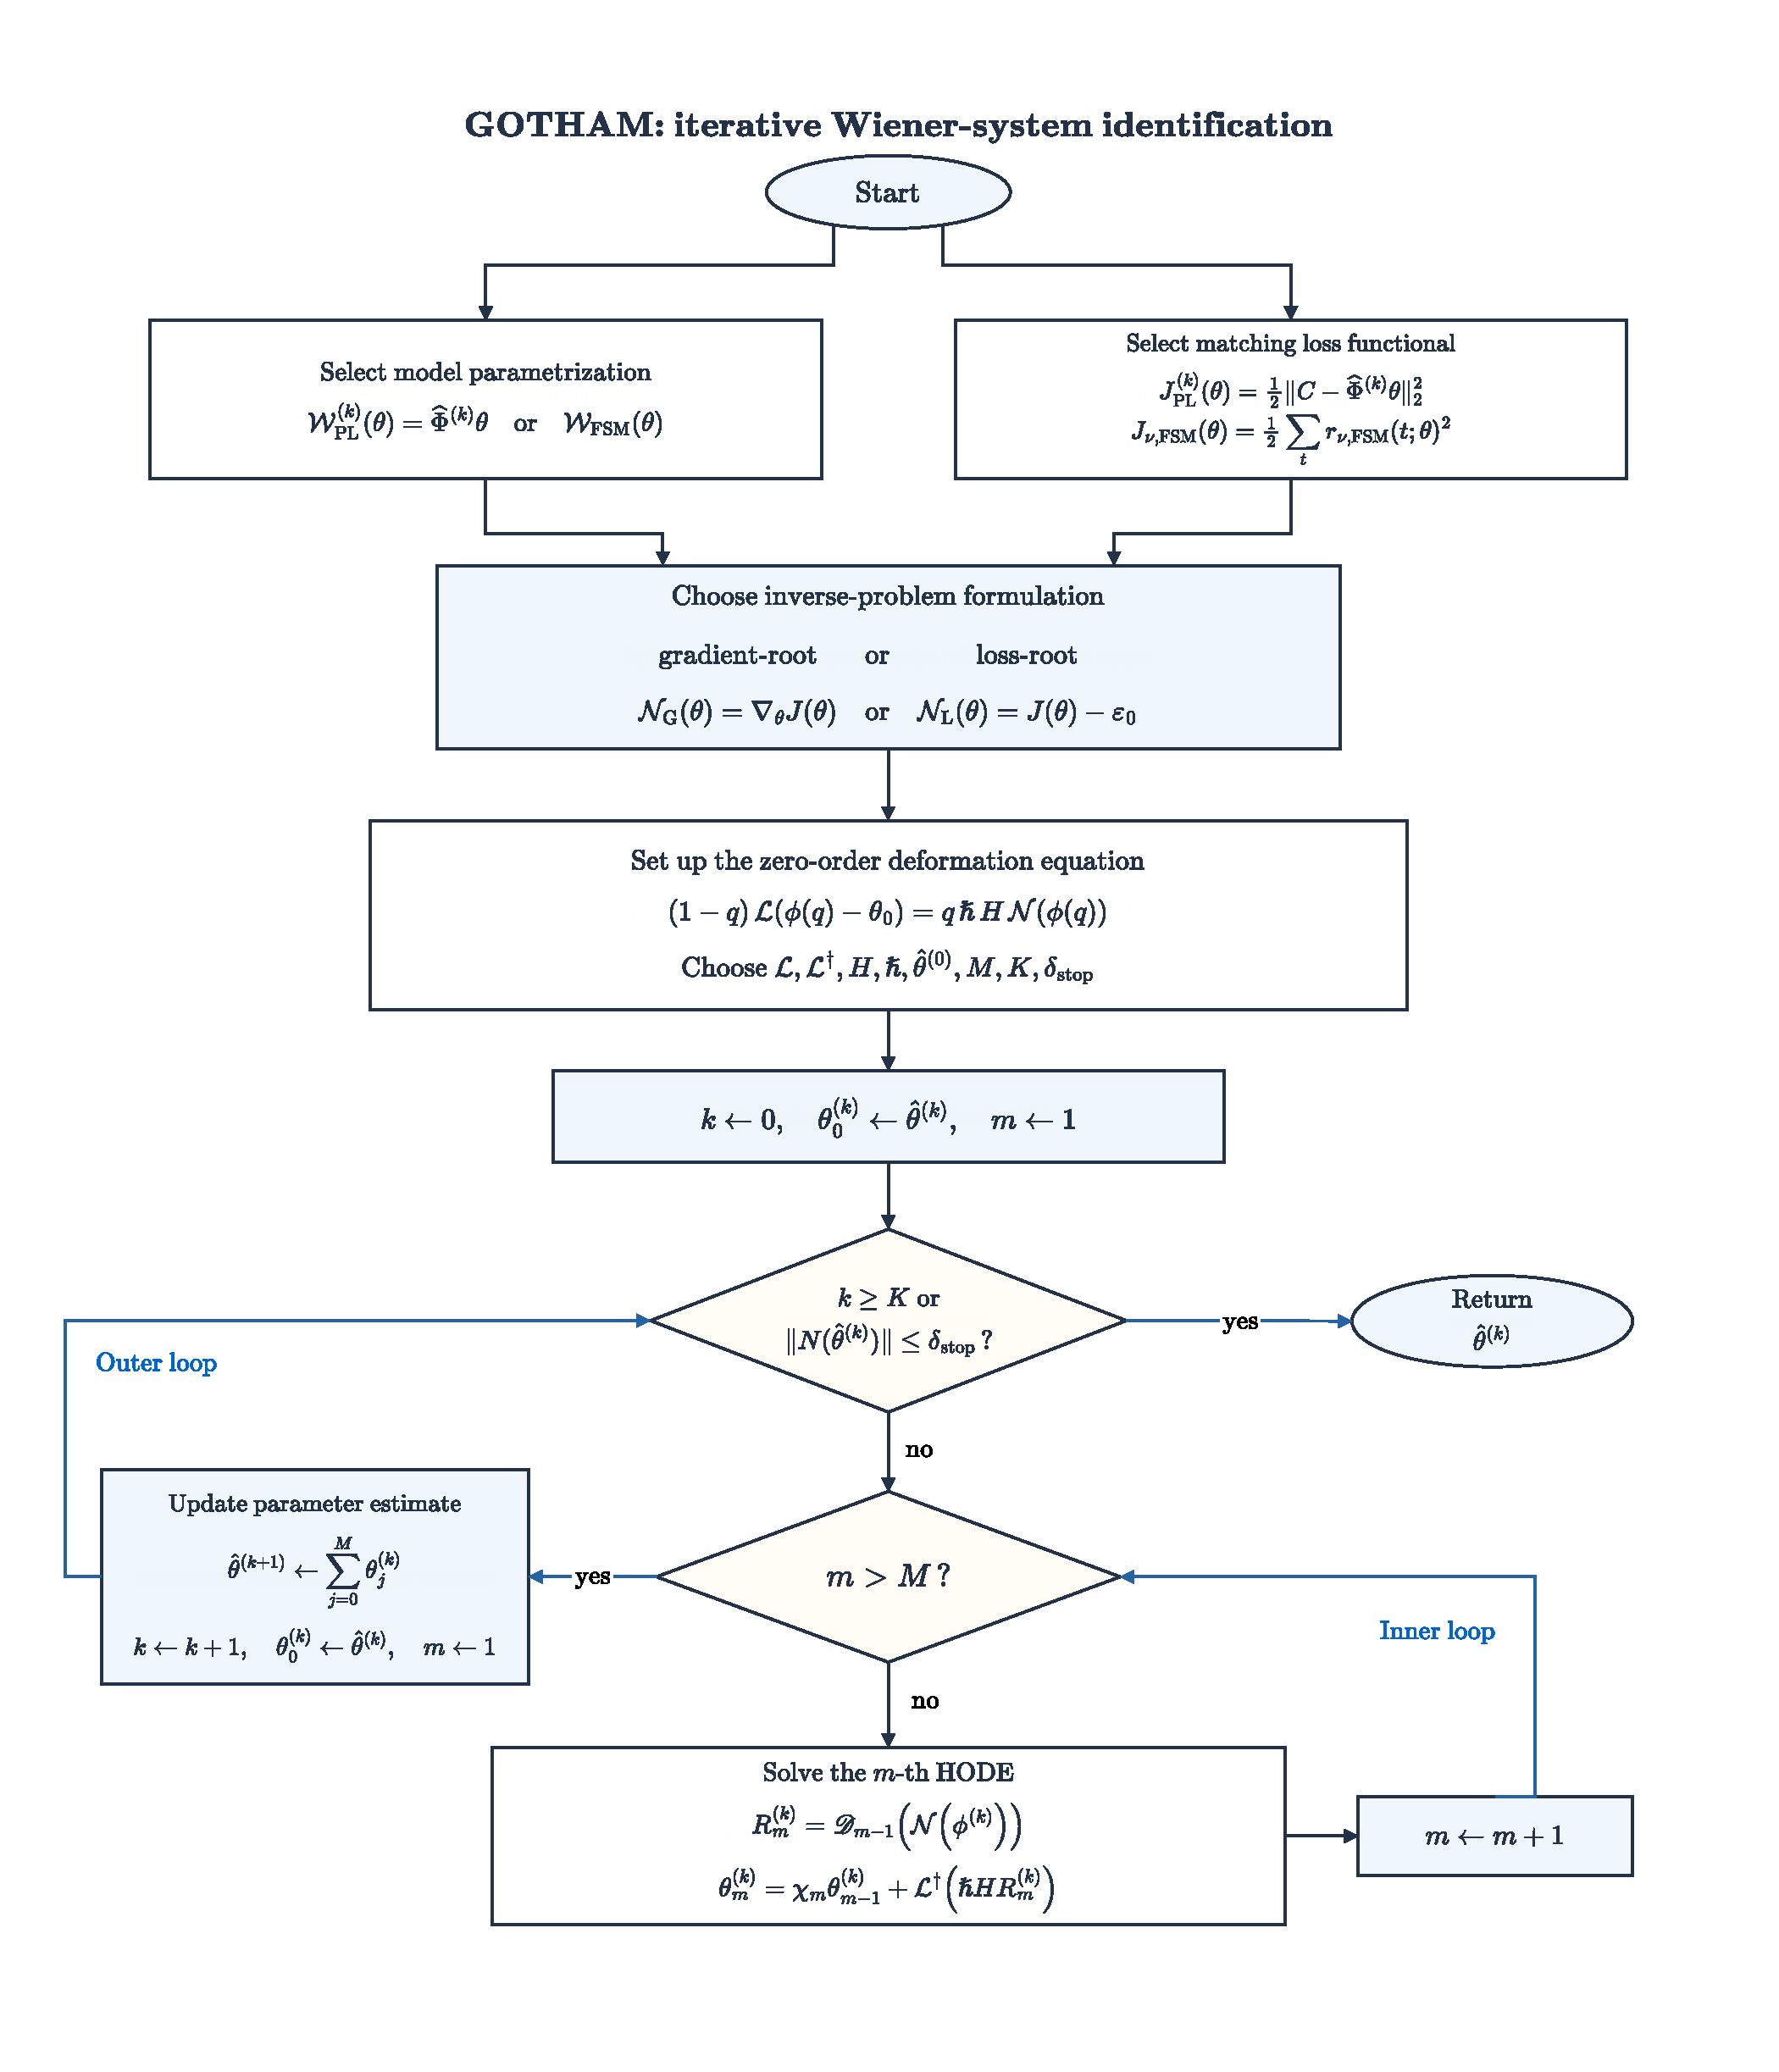
\includegraphics[width=\textwidth,height=.85\textheight,keepaspectratio]
       {figs/GOTHAM_flowchart.pdf}
    \caption{Flowchart of the GOTHAM iterative parameter-identification
    procedure for a Wiener system with AR output noise.}
    \label{fig:GOTHAM_flowchart}
\end{figure}
}{}
\clearpage
\begin{thebibliography}{99}
\bibitem[13]{Lv2026}
L. Lv, Y. Zhang, Y. Wu, C. Xu, Z. Li, and H. Yan,
Parameter estimation of Wiener nonlinear systems based on gradient iteration
theory and zebra optimization algorithm,
\emph{Journal of the Franklin Institute} 363 (2026), 108499.
\bibitem[16]{Wang2020}
Z. Wang, H. An, and X. Luo,
Adaptive filtering-based recursive identification for time-varying Wiener
output-error systems with unknown noise statistics,
\emph{Journal of the Franklin Institute} 357 (2020), 1280--1298.
\bibitem[36]{Polyak1969}
B. T. Polyak, Minimization of unsmooth functionals,
\emph{USSR Computational Mathematics and Mathematical Physics}
9 (1969), 14--29.
\end{thebibliography}
\end{document}
